\chapter{Results and Discussion}
The table below gives the answer to each research question and the strength of its evidence, which the following sections present in detail.


\begingroup\footnotesize\setlength{\tabcolsep}{4pt}
\begin{longtable}{>{\raggedright\arraybackslash}p{30.9mm}>{\raggedright\arraybackslash}p{38.3mm}>{\raggedright\arraybackslash}p{36.4mm}>{\raggedright\arraybackslash}p{33.2mm}}
\toprule
\textbf{Question} & \textbf{Answer} & \textbf{Key evidence} & \textbf{Strength} \\
\midrule
\endhead
RQ1: Does lower precision save energy per token? & Depends on the implementation: not on bitsandbytes with adapters attached; yes on vLLM & Stack A 4-bit about equal, 8-bit about 1.8-1.9 times float16; Stack B saves 36-38\% (FP8) and 64\% (AWQ) & Strong for Stack B. Provisional for Stack A pending an adapter-free run \\*
RQ2: What accuracy does it cost? & Not resolved for arithmetic; no clear cost elsewhere at 8B & tinyGSM8k falls 7.2 and 14.1 points under flexible scoring and 6.6 and 5.7 under strict scoring; the fall is not reproduced by coarser paired per-prompt data & Weak: 100 items per task and one run \\*
RQ3: Is measurement reliable on a shared node? & Not without monitoring & float16 ranged from 1.59 to 12.97 J/token, and three safeguards accepted it & Strong for the failure; cause not isolated \\*
RQ4: Can complexity routing beat the best static tier? & No, for these features and pools & Fuzzy matches random at all tested cuts; features predict sensitivity at about chance level & Strong for energy; proxy limits accuracy conclusions \\*
\bottomrule\noalign{\nobreak}
\end{longtable}
\addtocounter{table}{-1}
\endgroup

\section{Stack A: bitsandbytes with attached adapters}
With an adapter attached to every tier, 4-bit used about the same energy per token as float16, and 8-bit about 1.8 to 1.9 times as much, in three clean runs that agree closely.


\begingroup\footnotesize\setlength{\tabcolsep}{4pt}
\begin{longtable}{>{\raggedright\arraybackslash}p{32.4mm}>{\raggedright\arraybackslash}p{42.3mm}>{\raggedright\arraybackslash}p{29.6mm}>{\raggedright\arraybackslash}p{34.5mm}}
\caption[Llama-3.2-1B at batch 1, runs 5 / 6 / 7]{Llama-3.2-1B at batch 1, runs 5 / 6 / 7. Medians over prompts with at least 16 generated tokens (371 for 4-bit, 469 for 8-bit, 447 for 16-bit).}\\
\toprule
\textbf{Tier} & \textbf{Throughput (tokens/s)} & \textbf{Mean power (W)} & \textbf{Energy (J/token)} \\
\midrule
\endfirsthead
\toprule
\textbf{Tier} & \textbf{Throughput (tokens/s)} & \textbf{Mean power (W)} & \textbf{Energy (J/token)} \\
\midrule
\endhead
16-bit float16 & 80.7 / 81.8 / 81.5 & 136 / 142 / 130 & 1.69 / 1.73 / 1.59 \\*
8-bit LLM.int8 & 29.0 / 29.4 / 29.6 & 91 / 91 / 90 & 3.12 / 3.10 / 3.06 \\*
4-bit NF4 & 56.4 / 56.5 / 57.4 & 96 / 97 / 96 & 1.71 / 1.71 / 1.66 \\*
\bottomrule\noalign{\nobreak}
\end{longtable}
\endgroup

The difference between 4-bit and float16 changes sign across runs (+1.3\%, -1.5\%, +4.4\%), so we report the two as about equal. On the 367 prompts where every tier gave at least 16 tokens and a non-zero reading, the ratio of total energy per token was 1.007, 0.965 and 1.065. Each run's interval excludes 1.0, but the differences between runs are larger than the prompt-level intervals.

Among the tiers, float16 draws the most power but is also the fastest. The quantized tiers draw less power but run 1.4 times (4-bit) and 2.8 times (8-bit) slower, and the extra time costs more than the lower power saves.

Memory is a separate benefit. Weights occupy 2.47 GB in float16 (measured), and by calculation about 1.5 GB at 8-bit and 1.0 GB at 4-bit, because the tied embedding remains in float16.

\subsection*{Impact of LoRA adapters on energy measurements}
 The clean runs attach an unmerged LoRA adapter to every tier, with the largest rank on 4-bit. The only adapter-free energy data come from Session 1, whose float16 phase was disrupted.


\begingroup\footnotesize\setlength{\tabcolsep}{4pt}
\begin{longtable}{>{\raggedright\arraybackslash}p{34.5mm}>{\raggedright\arraybackslash}p{52.7mm}>{\raggedright\arraybackslash}p{54.3mm}}
\caption[Stack A with and without adapters]{Stack A with and without adapters. Session 1 values are pooled medians from tier\_\allowbreak{}medians.csv. The sessions also differ in date and possibly in GPU unit.}\\
\toprule
\textbf{Tier} & \textbf{Session 1, no adapters: tokens/s, W, J/token} & \textbf{Runs 5-7, adapters attached: tokens/s, W, J/token} \\
\midrule
\endfirsthead
\toprule
\textbf{Tier} & \textbf{Session 1, no adapters: tokens/s, W, J/token} & \textbf{Runs 5-7, adapters attached: tokens/s, W, J/token} \\
\midrule
\endhead
4-bit NF4 & 67.5, 90, 1.34 & 56.4-57.4, 96-97, 1.66-1.71 \\*
8-bit LLM.int8 & 26.9, 81, 3.02 & 29.0-29.6, 90-91, 3.06-3.12 \\*
16-bit float16 & 11.5, 85, 7.38 (disrupted, withdrawn) & 80.7-81.8, 130-142, 1.59-1.73 \\*
\bottomrule\noalign{\nobreak}
\end{longtable}
\endgroup

The adapter-free 4-bit tier is about 20\% faster and about 20\% cheaper per token than the adapted one, which is consistent with adapter overhead but does not prove it. We have no clean adapter-free float16 energy data. The adapter-free diagnostic reached 109.9 tokens/s, but it had no energy meter and used a different harness, so it cannot supply a J/token value. Whether bare bitsandbytes 4-bit matches float16 has therefore not been measured, and closing this gap requires one clean adapter-free run of all three tiers. The direction of the 8-bit result does agree with Poddar et al.~\cite{b6}, who attribute it to 16-bit computation.

\section{Per token versus per request}
Static 4-bit is 17-25\% cheaper per request than float16 even though it is no cheaper per token, because it generates less text.


\begingroup\footnotesize\setlength{\tabcolsep}{4pt}
\begin{longtable}{>{\raggedright\arraybackslash}p{26.3mm}>{\raggedright\arraybackslash}p{25.7mm}>{\raggedright\arraybackslash}p{28.7mm}>{\raggedright\arraybackslash}p{31.0mm}>{\raggedright\arraybackslash}p{24.3mm}}
\caption[Stack A, all 500 prompts]{Stack A, all 500 prompts.}\\
\toprule
\textbf{Tier} & \textbf{Mean tokens per response} & \textbf{Responses of 2 tokens or fewer (of 500)} & \textbf{Energy (J/request, runs 5 / 6 / 7)} & \textbf{Proxy accuracy} \\
\midrule
\endfirsthead
\toprule
\textbf{Tier} & \textbf{Mean tokens per response} & \textbf{Responses of 2 tokens or fewer (of 500)} & \textbf{Energy (J/request, runs 5 / 6 / 7)} & \textbf{Proxy accuracy} \\
\midrule
\endhead
16-bit float16 & 98.5 & 48 & 166 / 174 / 155 & 0.162 \\*
8-bit LLM.int8 & 103.4 & 30 & 323 / 320 / 317 & 0.186 \\*
4-bit NF4 & 76.5 & 122 & 130 / 130 / 129 & 0.110 \\*
\bottomrule\noalign{\nobreak}
\end{longtable}
\endgroup

The 4-bit tier's responses are 22\% shorter on average, it gives 2.5 times as many near-empty answers, and its proxy accuracy is 5.2 points lower. Its lower request energy therefore reflects less output and fewer correct answers, and is not an efficiency gain. Because token and request energy can move separately, as Vellaisamy et al. warn~\cite{b8}, we report both.

\section{Stack B: vLLM tiers save energy per token}
With vLLM, FP8 and AWQ 4-bit save energy at both batch sizes. Across the three runs, J/token agreed within 2\% for every 8B configuration and within 4.1\% for the 1B configurations.


\begingroup\footnotesize\setlength{\tabcolsep}{4pt}
\begin{longtable}{>{\raggedright\arraybackslash}p{14.7mm}>{\raggedright\arraybackslash}p{21.7mm}>{\raggedright\arraybackslash}p{13.4mm}>{\raggedright\arraybackslash}p{17.8mm}>{\raggedright\arraybackslash}p{18.0mm}>{\raggedright\arraybackslash}p{16.7mm}>{\raggedright\arraybackslash}p{28.0mm}}
\caption[Stack B, medians over three runs]{Stack B, medians over three runs. Saving is the median of per-run savings. The interval is the envelope of the three runs' 95\% paired bootstrap intervals.}\\
\toprule
\textbf{Model} & \textbf{Tier} & \textbf{Batch} & \textbf{J/token} & \textbf{Tokens/s} & \textbf{Mean power (W)} & \textbf{Saving vs float16 [95\% CI]} \\
\midrule
\endfirsthead
\toprule
\textbf{Model} & \textbf{Tier} & \textbf{Batch} & \textbf{J/token} & \textbf{Tokens/s} & \textbf{Mean power (W)} & \textbf{Saving vs float16 [95\% CI]} \\
\midrule
\endhead
1B & float16 & 1 & 0.945 & 307 & 290 & Baseline \\*
1B & FP8 & 1 & 0.604 & 413 & 249 & 36\% [34, 39] \\
8B & float16 & 1 & 5.311 & 56 & 298 & Baseline \\
8B & FP8 & 1 & 3.299 & 87 & 287 & 38\% [38, 38] \\
8B & AWQ 4-bit & 1 & 1.887 & 158 & 298 & 64\% [64, 65] \\
1B & float16 & 8 & 0.139 & 1989 & 275 & Baseline \\
1B & FP8 & 8 & 0.087 & 2743 & 238 & 37\% [36, 39] \\
8B & float16 & 8 & 0.679 & 435 & 296 & Baseline \\*
8B & FP8 & 8 & 0.423 & 673 & 285 & 38\% [37, 38] \\*
8B & AWQ 4-bit & 8 & 0.245 & 1196 & 292 & 64\% [64, 65] \\*
\bottomrule\noalign{\nobreak}
\end{longtable}
\endgroup

\begin{figure}[htbp]
\centering
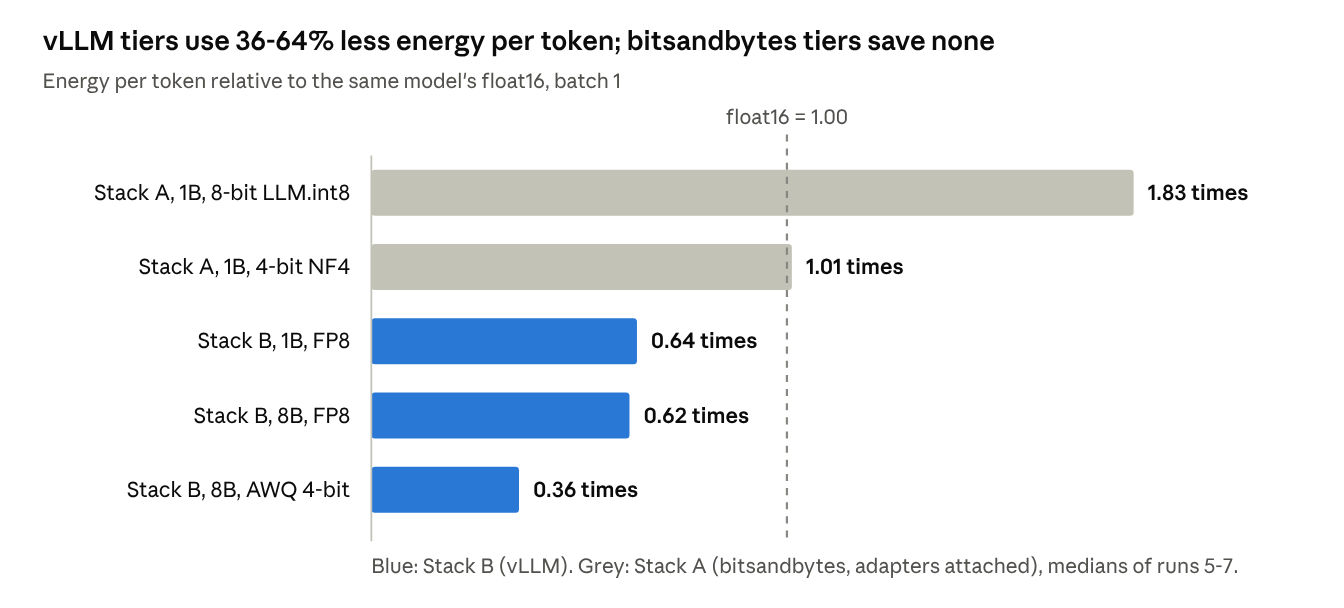
\includegraphics[width=\linewidth]{figs/fig_relative_energy.png}
\caption[Energy per token relative to the same model's float16 at batch 1: vLLM tiers use 36-64\% less, bitsandbytes tiers save none]{Energy per token relative to the same model's float16 at batch 1: vLLM tiers use 36-64\% less, bitsandbytes tiers save none. Source: paper/results.md and paper/analysis/session5\_\allowbreak{}summary.csv; ratios computed from the medians in Tables 5.1 and 5.4.}
\end{figure}
We compare each tier with float16 on its own stack, because the stacks differ in GPU unit, driver, time of day and adapter use. At 8B almost every response reached the 128-token cap on all tiers (mean 127.7 to 127.9 tokens in run 2), so these savings do not come from shorter answers.

\textbf{Why the stacks differ.} Energy is power multiplied by time, and at 8B the power is nearly constant, so the saving comes from time. At batch 1, throughput rises 1.55 times with FP8 and 2.8 times with AWQ, compared with 2 times and 4 times fewer weight bytes. At 1B, FP8 is 1.35 times faster.

\begin{figure}[htbp]
\centering
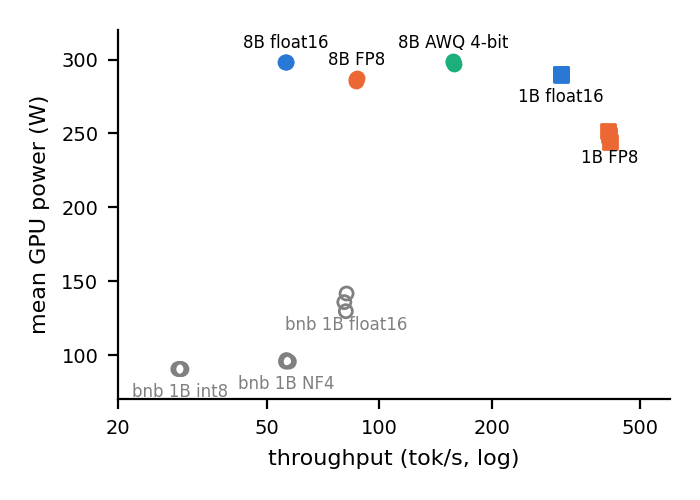
\includegraphics[width=\linewidth]{figs/fig_why.png}
\caption[Throughput and mean power at batch 1]{Throughput and mean power at batch 1.}
\end{figure}
A plausible mechanism is memory traffic: small-batch decoding may be limited by reading weights once per token, and these kernels read fewer bytes and operate on them directly~\cite{b44}. This fits the throughput and power data, but we did not measure memory traffic, so the explanation remains a hypothesis. The design also cannot separate kernel from engine, because vLLM's float16 differs from Stack A's float16 as well.

\textbf{Batch size and stack.} Moving from batch 1 to batch 8 reduces J/token by 6.8 to 7.8 times for every tier, while the relative savings of FP8 and AWQ remain unchanged. vLLM's float16 at 1B is about 41-45\% cheaper per token than Stack A's float16. That comparison crosses GPU units, drivers, times of day and adapter use, and the J/token definitions differ, so it is indicative only.

\textbf{Comparison with prior work.} The following table sets these results beside published figures.


\begingroup\footnotesize\setlength{\tabcolsep}{4pt}
\begin{longtable}{>{\raggedright\arraybackslash}p{36.3mm}>{\raggedright\arraybackslash}p{33.4mm}>{\raggedright\arraybackslash}p{33.1mm}>{\raggedright\arraybackslash}p{36.0mm}}
\caption[Comparison with published results]{Comparison with published results.}\\
\toprule
\textbf{Source} & \textbf{Reported result} & \textbf{This thesis} & \textbf{Assessment} \\
\midrule
\endfirsthead
\toprule
\textbf{Source} & \textbf{Reported result} & \textbf{This thesis} & \textbf{Assessment} \\
\midrule
\endhead
Poddar et al.~\cite{b6} & bitsandbytes almost 2 times at equal batch size & 8-bit about 1.8-1.9 times; 4-bit about 1.0 times with adapters & Agrees for 8-bit. 4-bit is lower, on a different GPU, tools and workload \\*
Basta~\cite{b47} & bitsandbytes int8 saves up to 4 times against FP32 on short generation & 8-bit costs more than float16 in decode-heavy use & Not a direct conflict: FP32 baseline and prefill-heavy case. Not tested here \\*
TokenPowerBench~\cite{b7} & FP8 saves about 30\% at 405B & FP8 saves 36-38\% at 1B and 8B & Same direction; very different scale and hardware \\*
TokenPowerBench~\cite{b7} & vLLM 25-40\% below Transformers & 41-45\% at 1B, float16 & Same direction; the thesis figure is confounded \\*
Vellaisamy et al.~\cite{b8} & Token and request energy can diverge & 4-bit equal per token, cheaper per request & Agrees \\*
\bottomrule\noalign{\nobreak}
\end{longtable}
\endgroup

\section{Accuracy}
We trust the accuracy evidence less than the energy evidence: each benchmark has 100 items and each configuration ran once, so only large differences can be interpreted.


\begingroup\footnotesize\setlength{\tabcolsep}{4pt}
\begin{longtable}{>{\raggedright\arraybackslash}p{14.0mm}>{\raggedright\arraybackslash}p{38.1mm}>{\raggedright\arraybackslash}p{24.3mm}>{\raggedright\arraybackslash}p{33.5mm}>{\raggedright\arraybackslash}p{26.2mm}}
\caption[tinyBenchmarks, 100 items per task, one run per configuration]{tinyBenchmarks, 100 items per task, one run per configuration.}\\
\toprule
\textbf{Stack} & \textbf{Configuration} & \textbf{tinyMMLU} & \textbf{tinyHellaswag} & \textbf{tinyGSM8k} \\
\midrule
\endfirsthead
\toprule
\textbf{Stack} & \textbf{Configuration} & \textbf{tinyMMLU} & \textbf{tinyHellaswag} & \textbf{tinyGSM8k} \\
\midrule
\endhead
A & 1B float16 & 0.433 & 0.636 & 0.062 \\*
A & 1B float16 + adapter & 0.400 & 0.623 & 0.061 \\
A & 1B 8-bit & 0.391 & 0.634 & 0.104 \\
A & 1B 8-bit + adapter & 0.388 & 0.640 & 0.075 \\
A & 1B 4-bit & 0.393 & 0.573 & 0.063 \\
A & 1B 4-bit + adapter & 0.368 & 0.594 & 0.041 \\
B & 1B float16 & 0.433 & 0.629 & 0.092 \\
B & 1B FP8 & 0.380 & 0.624 & 0.084 \\
B & 8B float16 & 0.629 & 0.818 & 0.746 \\*
B & 8B FP8 & 0.640 & 0.823 & 0.674 \\*
B & 8B AWQ 4-bit & 0.663 & 0.802 & 0.605 \\*
\bottomrule\noalign{\nobreak}
\end{longtable}
\endgroup

\begin{figure}[htbp]
\centering
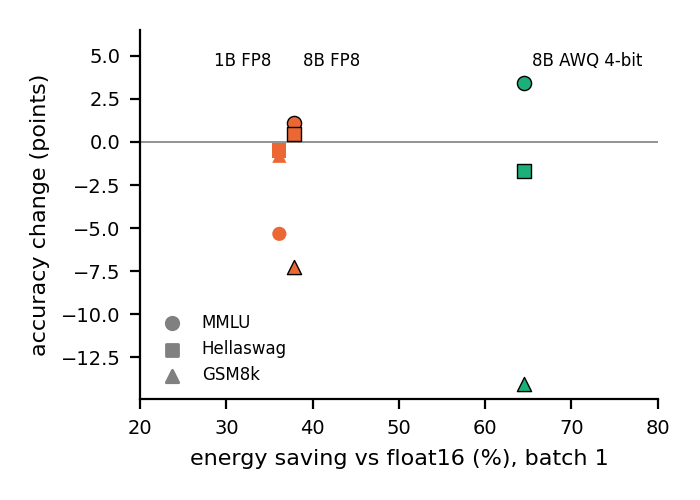
\includegraphics[width=\linewidth]{figs/fig_tradeoff.png}
\caption[Energy saving versus accuracy change]{Energy saving versus accuracy change. Black-edged markers are 8B; plain markers are 1B.}
\end{figure}
At 8B, FP8 and AWQ stay within 3.5 points of float16 on tinyMMLU and tinyHellaswag, in both directions. At 1B, FP8 loses 5.3 points on tinyMMLU and under 1 point on the others. tinyGSM8k scores of 4-10\% are near the floor for this base model, so differences there carry little information.

\textbf{The size of any arithmetic loss is not established.} Under flexible scoring, tinyGSM8k falls by 7.2 points with FP8 and 14.1 points with AWQ. Three checks qualify this.


\begingroup\footnotesize\setlength{\tabcolsep}{4pt}
\begin{longtable}{>{\raggedright\arraybackslash}p{35.5mm}>{\raggedright\arraybackslash}p{20.8mm}>{\raggedright\arraybackslash}p{25.1mm}>{\raggedright\arraybackslash}p{27.1mm}>{\raggedright\arraybackslash}p{27.5mm}}
\caption[tinyGSM8k under two scoring rules, in points]{tinyGSM8k under two scoring rules, in points.}\\
\toprule
\textbf{Configuration} & \textbf{Strict match} & \textbf{Flexible extract} & \textbf{Change from float16: strict} & \textbf{Change from float16: flexible} \\
\midrule
\endfirsthead
\toprule
\textbf{Configuration} & \textbf{Strict match} & \textbf{Flexible extract} & \textbf{Change from float16: strict} & \textbf{Change from float16: flexible} \\
\midrule
\endhead
8B float16 & 0.634 & 0.746 & Baseline & Baseline \\*
8B FP8 & 0.568 & 0.674 & -6.6 & -7.2 \\*
8B AWQ 4-bit & 0.577 & 0.605 & -5.7 & -14.1 \\*
\bottomrule\noalign{\nobreak}
\end{longtable}
\endgroup


\begingroup\footnotesize\setlength{\tabcolsep}{4pt}
\begin{longtable}{>{\raggedright\arraybackslash}p{35.2mm}>{\raggedright\arraybackslash}p{23.9mm}>{\raggedright\arraybackslash}p{39.6mm}>{\raggedright\arraybackslash}p{40.1mm}}
\caption[Paired proxy accuracy at 8B, Stack B run 2, in points]{Paired proxy accuracy at 8B, Stack B run 2, in points. Source: thesis\_\allowbreak{}s5\_\allowbreak{}by\_\allowbreak{}source.csv.}\\
\toprule
\textbf{Source dataset} & \textbf{Prompts} & \textbf{FP8 minus float16 [95\% CI]} & \textbf{AWQ minus float16 [95\% CI]} \\
\midrule
\endfirsthead
\toprule
\textbf{Source dataset} & \textbf{Prompts} & \textbf{FP8 minus float16 [95\% CI]} & \textbf{AWQ minus float16 [95\% CI]} \\
\midrule
\endhead
All & 500 & +0.8 [-1.6, +3.2] & -1.4 [-4.6, +1.6] \\*
TriviaQA & 200 & -1.5 [-6.5, +3.0] & -5.0 [-10.5, 0.0] \\*
Alpaca & 150 & 0.0 [-4.7, +4.0] & +1.3 [-2.7, +5.3] \\*
GSM8K & 75 & +6.7 [0.0, +13.3] & -2.7 [-10.7, +6.7] \\*
CodeAlpaca & 75 & +2.7 [0.0, +6.7] & +4.0 [-2.7, +12.0] \\*
\bottomrule\noalign{\nobreak}
\end{longtable}
\endgroup

\begin{enumerate}
\item \textbf{Sampling noise.} As a rough guide, if the scores are treated as independent proportions on 100 items, the standard error of a difference is about 6.5 points. On that basis FP8's loss is about 1.1 standard errors and AWQ's about 2.2, which passes the usual two-standard-error threshold. This is an approximation, since items are shared and scores are IRT-weighted, and no formal test was possible because per-item outputs were not retained.
\item \textbf{Scoring rule.} AWQ's loss falls from 14.1 to 5.7 points under strict matching (Table 5.7), so much of that gap depends on answer format. FP8's loss barely changes (7.2 to 6.6 points), and both tiers remain below float16 under strict matching.
\item \textbf{Independent items.} On the 75 GSM8K prompts in the evaluation set, FP8 is 6.7 points higher and AWQ's difference includes zero (Table 5.8). This check is limited: the proxy only requires the final number to appear in the output, and responses are capped at 128 tokens.
\end{enumerate}
The evidence therefore allows an arithmetic penalty at AWQ without fixing its size. The paired interval excludes a 14-point loss but includes one of about 6 points, on a coarser measure. On TriviaQA, AWQ's interval of -10.5 to 0.0 points means a smaller factual-recall cost cannot be ruled out either. A full GSM8K evaluation with per-item outputs is needed to resolve the question.

Outputs also change more than scores suggest. Compared with float16, only 18-19\% of answers are identical at 1B FP8, about 7\% at 8B FP8 and 1\% at 8B AWQ. A deployment that needs stable answers should test for this directly.

\textbf{LoRA adapters did not help.} They lower tinyMMLU at every tier and tinyGSM8k at both quantized tiers, with mixed effects on tinyHellaswag. Most differences are a few points and within noise. All three were trained on the 4-bit model (section 3.7), so this does not rule out properly tier-specific training.

\section{A measurement pitfall on a shared node}
The same float16 model consumed between 1.59 and 12.97 J/token across Stack A measurements, while answers and routing decisions stayed the same. Three safeguards accepted the inflated readings.


\begingroup\footnotesize\setlength{\tabcolsep}{4pt}
\begin{longtable}{>{\raggedright\arraybackslash}p{30.3mm}>{\raggedright\arraybackslash}p{23.9mm}>{\raggedright\arraybackslash}p{19.9mm}>{\raggedright\arraybackslash}p{23.5mm}>{\raggedright\arraybackslash}p{15.9mm}>{\raggedright\arraybackslash}p{19.9mm}}
\caption[Stack A float16 across measurements]{Stack A float16 across measurements. Medians over prompts with at least 16 tokens.}\\
\toprule
\textbf{Measurement} & \textbf{GPU unit} & \textbf{Start (IST)} & \textbf{Tokens/s} & \textbf{Mean power (W)} & \textbf{J/token} \\
\midrule
\endfirsthead
\toprule
\textbf{Measurement} & \textbf{GPU unit} & \textbf{Start (IST)} & \textbf{Tokens/s} & \textbf{Mean power (W)} & \textbf{J/token} \\
\midrule
\endhead
Session 1, three runs, no adapters & Not recorded & 4 Sep & 10.5-11.8 & 85 & 7.2-7.8 \\*
Run 4 & c53791fb & 29 Sep, 11:48 & 6.2 & 81 & 12.97 \\*
Run 5 & da9c4cd1 & 30 Sep, 00:05 & 80.7 & 136 & 1.69 \\*
Run 6 & da9c4cd1 & 1 Oct, 00:58 & 81.8 & 142 & 1.73 \\*
Run 7 & da9c4cd1 & 3 Oct, 00:57 & 81.5 & 130 & 1.59 \\*
\bottomrule\noalign{\nobreak}
\end{longtable}
\endgroup

\begin{figure}[htbp]
\centering
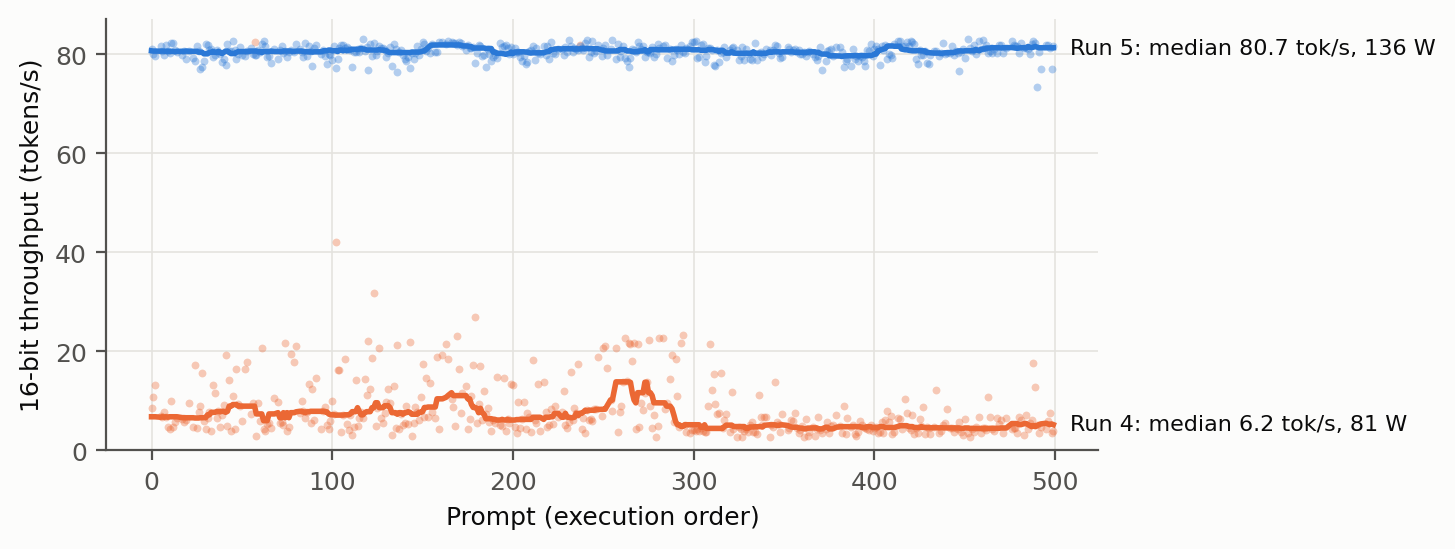
\includegraphics[width=\linewidth]{figs/fig_disruption.png}
\caption[Float16 throughput per prompt in a disrupted run (run 4) and a clean run (run 5)]{Float16 throughput per prompt in a disrupted run (run 4) and a clean run (run 5). Lines are rolling medians over 25 prompts. The two runs used different GPU units.}
\end{figure}
\textbf{Signature of disruption.} Clean float16 runs are fast and power-hungry, whereas disrupted runs are slow and low-power, near the GPU's mostly-idle draw. A waiting GPU still draws substantial power, so energy per token rises roughly with the slowdown.

\textbf{A host-side slowdown.} We ran a diagnostic that timed plain float16 generation with no router, adapters or energy meter. In daytime it ran at a mean of 8.5 tokens/s (range 4.4-25.6), with GPU SM utilization of 0\% at the median and 25\% at the 90th percentile, and CPU time equal to wall time. At night it ran at 109.9 tokens/s with a 1.01 times spread. We interpret this as the GPU waiting on a slowed CPU-side launch path. Because the process stayed on the CPU, the diagnostic alone cannot separate contention from additional work within the software stack, and we did not isolate the mechanism.

Disruption is not specific to 16-bit. In run 2, which interleaved tiers under known load, 16-bit stayed within 1.6\% (as recorded in the experiment log) while 4-bit and 8-bit were inflated 3 to 5 times. In by-tier runs, 16-bit ran last.

\textbf{Why the safeguards missed it.}


\begingroup\footnotesize\setlength{\tabcolsep}{4pt}
\begin{longtable}{>{\raggedright\arraybackslash}p{34.7mm}>{\raggedright\arraybackslash}p{46.5mm}>{\raggedright\arraybackslash}p{60.4mm}}
\toprule
\textbf{Safeguard} & \textbf{What it checks} & \textbf{Why it failed} \\
\midrule
\endhead
End-of-run co-tenant snapshot & Other processes on the GPU, once & Taken at a single moment, and the GPU was not the contended resource. It was empty for run 4 and for runs later confirmed contended. \\*
Repeat-run agreement & Session 1's three runs agreed within 6.6\% & They ran back-to-back under the same conditions. Agreement measured consistency, not cleanliness. Their 16-bit mean of 8.124 J/token is withdrawn; the same 1,500 rows give per-run medians of 7.2 to 7.8 and a pooled median of 7.38. \\*
Automated validator & Completeness, positivity, plausibility, oracle consistency & A uniform slowdown stays inside every limit. The experiment log records that verify\_\allowbreak{}results.py passed run 4. \\*
\bottomrule\noalign{\nobreak}
\end{longtable}
\addtocounter{table}{-1}
\endgroup

\textbf{What the evidence does and does not establish.} Time of day and GPU unit are fully confounded in Stack A: runs 1-4 all used c53791fb and all showed contention or disruption, while clean runs 5-7 all used da9c4cd1, and the diagnostics did not record a UUID. Run 4's 4-bit and 8-bit tiers also drew about 9\% less power than the clean runs at similar throughput, which may reflect a unit or a time effect.

Stack B ran on c53791fb in daytime, at run-median host load of 1.6 to 6, with 100\% median GPU utilization in 29 of 30 configuration-runs and steady throughput. This unit is therefore not simply faulty, although the comparison is not a clean test, because vLLM's CUDA graphs should need far less CPU work per token, and Stack B was not repeated at night or on the other unit.

The evidence supports three claims: float16 readings differed by a factor of about 8 between their extremes, and by 7.7 between run 4 and run 5; three safeguards accepted them; and throughput with power exposed them. It does not support the claim that time of day caused the slowdown. A short diagnostic on each unit, by day and by night, with the UUID recorded, would settle it.

\textbf{Monitoring protocol.} We derived the protocol below from this failure, and Stack B follows it; none of its 30 configuration-runs was flagged. The 20\% throughput rule compares a run with its own configuration's median, so it could miss a slowdown shared by every run: Session 1's float16 runs were all within about 4\% of their median. Continuous GPU utilization is therefore the more independent check.

\begin{enumerate}
\item Report throughput and mean power alongside J/token.
\item Check throughput stability across the run, not only the final mean.
\item Sample GPU utilization, co-tenants, host load and CPU clock continuously, every 2 s.
\item Record the GPU UUID and bus ID for every run, including diagnostics.
\item Flag and re-measure any configuration that departs from its clean baseline by over 20\%.
\item Add a watchdog: one Stack B configuration hung while loading, with the engine at 100\% CPU and the GPU idle.
\end{enumerate}
\section{Routing evaluation}
The fuzzy router did not beat a random router with the same mix on either stack, and it did not beat the best static tier.

\textbf{Stack A.} The table below compares the policies on all 500 prompts.


\begingroup\footnotesize\setlength{\tabcolsep}{4pt}
\begin{longtable}{>{\raggedright\arraybackslash}p{51.3mm}>{\raggedright\arraybackslash}p{38.3mm}>{\raggedright\arraybackslash}p{52.0mm}}
\caption[Stack A routing on 500 prompts]{Stack A routing on 500 prompts. Accuracy is identical across runs because decoding is deterministic.}\\
\toprule
\textbf{Policy} & \textbf{Proxy accuracy} & \textbf{J/request (runs 5 / 6 / 7)} \\
\midrule
\endfirsthead
\toprule
\textbf{Policy} & \textbf{Proxy accuracy} & \textbf{J/request (runs 5 / 6 / 7)} \\
\midrule
\endhead
Static 4-bit & 0.110 & 130 / 130 / 129 \\*
Static 8-bit & 0.186 & 323 / 320 / 317 \\*
Static 16-bit & 0.162 & 166 / 174 / 155 \\*
Fuzzy router & 0.156 & 238 / 239 / 232 \\*
Random, matched mix & 0.166 & 241 / 242 / 234 \\*
Threshold on mean feature & 0.120 & 185 / 184 / 182 \\*
Oracle & 0.258 & 140 / 141 / 134 \\*
\bottomrule\noalign{\nobreak}
\end{longtable}
\endgroup

A paired bootstrap of fuzzy minus static 16-bit gives +71.7 J/request (95\% CI 61.0-82.2), +65.4 (54.9-75.8) and +76.4 (66.5-86.9) in runs 5, 6 and 7. That is 38-49\% more energy, with an accuracy difference of -0.006 (CI -0.034 to +0.020 in runs 5 and 6, and -0.032 to +0.020 in run 7).

In run 5 the sensor sends 61\% of prompts labelled hard to 16-bit against 21\% of those labelled easy. Much of this comes from the code or maths flag, which is set on 73\% of hard prompts and 1\% of easy ones, so it largely recognizes the source dataset; with the flag off, the shares are 37.5\% and 20\%. The router also sends 52\% of all prompts to 8-bit, the most expensive tier. Its choice matches the oracle's on 23.6\% of prompts in run 5, inside the range for a matched random router (mean 25.9\%, 95\% band 22.4 to 29.4). Only 129 of the 500 prompts are answered correctly by any tier under the proxy, which limits what any router can gain.

\textbf{Stack B.} Tiers now differ in cost, so routing has something to save. Two pools were replayed at batch 1.


\begingroup\footnotesize\setlength{\tabcolsep}{4pt}
\begin{longtable}{>{\raggedright\arraybackslash}p{38.6mm}>{\raggedright\arraybackslash}p{26.3mm}>{\raggedright\arraybackslash}p{23.7mm}>{\raggedright\arraybackslash}p{23.2mm}>{\raggedright\arraybackslash}p{24.1mm}}
\caption[Stack B routing replay, run 1]{Stack B routing replay, run 1. Runs 2 and 3 are within 2 J/request, with identical accuracy.}\\
\toprule
\textbf{Policy} & \textbf{8B precision pool: J/request} & \textbf{Accuracy} & \textbf{1B vs 8B AWQ pool: J/request} & \textbf{Accuracy} \\
\midrule
\endfirsthead
\toprule
\textbf{Policy} & \textbf{8B precision pool: J/request} & \textbf{Accuracy} & \textbf{1B vs 8B AWQ pool: J/request} & \textbf{Accuracy} \\
\midrule
\endhead
Static cheapest (8B AWQ; 1B float16) & 240 & 0.350 & 104 & 0.164 \\*
Static 8B FP8 & 422 & 0.372 & Not in pool & Not in pool \\*
Static largest (8B float16; 8B AWQ) & 678 & 0.364 & 240 & 0.350 \\*
Fuzzy router & 477 & 0.368 & 221 & 0.322 \\*
Random, matched mix & 478 & 0.366 & 219 & 0.321 \\*
Learned, cross-fitted & Not run & Not run & 240 & 0.350 \\*
Oracle & 260 & 0.442 & 136 & 0.398 \\*
\bottomrule\noalign{\nobreak}
\end{longtable}
\endgroup

\begin{itemize}
\item \textbf{Precision pool.} Always serving AWQ costs 240 J/request against 678 for float16. Its accuracy gap to FP8 is within noise (-0.022, widest paired CI -0.054 to +0.010). The fuzzy router lands at 477 J, level with random, because it sends a third of prompts to float16 without picking the ones that need it.
\item \textbf{Model-size pool.} The fuzzy router saves 8\% against static 8B AWQ but loses 2.8 points (CI -4.8 to -1.0), again matching random.
\item \textbf{Learned baseline.} A logistic regression on the same five features always chose 8B at thresholds of 0.5 and above. This is a weak test, because the 1B model is correct on only 16.4\% of prompts, so its predicted probability rarely reaches 0.5. The cross-validated AUC of 0.58 in Table 5.13 is the more informative measure.
\item \textbf{Headroom.} In the model-size pool, the oracle would use 43\% less energy than always-8B-AWQ and gain 4.8 points. The oracle knows each outcome in advance and cannot be deployed, so this shows only that routing has headroom in principle. The feature tests below suggest that these surface features are unlikely to capture it.
\end{itemize}
\textbf{Sensitivity to tier cuts.} The negative result does not depend on the choice of 33/66.


\begingroup\footnotesize\setlength{\tabcolsep}{4pt}
\begin{longtable}{>{\raggedright\arraybackslash}p{14.1mm}>{\raggedright\arraybackslash}p{20.9mm}>{\raggedright\arraybackslash}p{19.8mm}>{\raggedright\arraybackslash}p{29.0mm}>{\raggedright\arraybackslash}p{20.1mm}>{\raggedright\arraybackslash}p{29.2mm}}
\caption[Fuzzy score replayed at other cuts, Stack A run 5 and Stack B run 2]{Fuzzy score replayed at other cuts, Stack A run 5 and Stack B run 2. The band is the central 95\% of 1,000 random permutations of the same tier assignment. Reference: static float16 on Stack A, 166 J at 0.162; static AWQ on Stack B, 241 J at 0.350. The 40/60 and 45/55 rows match because no scores fall between those cuts.}\\
\toprule
\textbf{Cuts} & \textbf{Mix, low/mid/high (\%)} & \textbf{Stack A: J/request} & \textbf{Stack A: accuracy [random band]} & \textbf{Stack B 8B: J/request} & \textbf{Stack B 8B: accuracy [random band]} \\
\midrule
\endfirsthead
\toprule
\textbf{Cuts} & \textbf{Mix, low/mid/high (\%)} & \textbf{Stack A: J/request} & \textbf{Stack A: accuracy [random band]} & \textbf{Stack B 8B: J/request} & \textbf{Stack B 8B: accuracy [random band]} \\
\midrule
\endhead
25/75 & 14.4 / 57.6 / 28.0 & 247 & 0.166 [0.152, 0.184] & 467 & 0.368 [0.350, 0.382] \\*
30/70 & 15.6 / 54.8 / 29.6 & 243 & 0.158 [0.150, 0.186] & 469 & 0.368 [0.350, 0.380] \\*
33/66 & 15.6 / 51.6 / 32.8 & 238 & 0.156 [0.148, 0.184] & 477 & 0.368 [0.350, 0.380] \\*
40/60 & 15.8 / 35.2 / 49.0 & 217 & 0.158 [0.146, 0.180] & 519 & 0.362 [0.350, 0.382] \\*
45/55 & 15.8 / 35.2 / 49.0 & 217 & 0.158 [0.146, 0.180] & 519 & 0.362 [0.350, 0.380] \\*
\bottomrule\noalign{\nobreak}
\end{longtable}
\endgroup

At every cut, accuracy falls inside the random band, and no cut reaches the energy of the cheaper reference on either stack. Stack B accuracy at each cut is 1.2 to 1.8 points above static AWQ, at about twice its energy.

These comparisons favour the router, if anything, because its ranges and edges were calibrated on the same 500 prompts.

\textbf{Why the router fails.} We tested the features directly against the outcomes they were intended to predict.


\begingroup\footnotesize\setlength{\tabcolsep}{4pt}
\begin{longtable}{>{\raggedright\arraybackslash}p{31.2mm}>{\raggedright\arraybackslash}p{21.9mm}>{\raggedright\arraybackslash}p{49.9mm}>{\raggedright\arraybackslash}p{35.8mm}}
\caption[Prediction by the five sensor features]{Prediction by the five sensor features. An AUC of 0.5 is chance. Values are from one cross-validation split. Source: thesis\_\allowbreak{}feature\_\allowbreak{}signal.csv.}\\
\toprule
\textbf{Target} & \textbf{Positive prompts} & \textbf{Largest absolute Spearman correlation} & \textbf{Cross-validated AUC} \\
\midrule
\endfirsthead
\toprule
\textbf{Target} & \textbf{Positive prompts} & \textbf{Largest absolute Spearman correlation} & \textbf{Cross-validated AUC} \\
\midrule
\endhead
Stack A: float16 right, 4-bit wrong & 44 & 0.070 (Flesch-Kincaid, p=0.12) & 0.51 \\*
Stack B 8B: float16 right, AWQ wrong & 34 & 0.091 (token length, p=0.042) & 0.43 \\*
Stack A: float16 correct & 81 & 0.070 (code or maths, p=0.12) & 0.52 \\*
Stack B 8B: float16 correct & 182 & 0.184 (code or maths, negative, p\textless{}0.001) & 0.65 \\*
Stack B 1B float16 correct & 82 & 0.122 (code or maths, negative, p=0.006) & 0.58 \\*
\bottomrule\noalign{\nobreak}
\end{longtable}
\endgroup

The two sensitivity targets are what a precision router needs to predict, and both sit at about chance level. The 0.43 is a product of the split: over 20 splits the mean AUC is 0.49 and 0.50, with single-split ranges of 0.43 to 0.53 and 0.45 to 0.54. Bootstrap intervals reach about 0.61, so weak signal is not excluded. The single p=0.042 correlation is one of ten tests on those targets and would not survive a Bonferroni correction.

The features do carry some signal about whether a prompt can be answered at all, mainly through the code or maths indicator, but this does not indicate which tier is sufficient. That distinction fits the router's behaviour: it responds to the difficulty labels and yet does not outperform random assignment. Although the analysis is limited by few positive cases and the proxy metric, the result agrees with GreenServ's ablation, where text complexity did not reduce regret~\cite{b48}, and is consistent with the finer-grained sensitivity reported by DP-LLM~\cite{b50}, although neither study tested this directly.



\section{Discussion}
Our founding assumption did not hold on the Stack A configuration tested: fewer stored bits did not yield less energy per token, because energy depends on execution time and power, not on storage alone. On Stack B, by contrast, savings were large and stable across runs. The following guidance applies within this study's scope:


\begingroup\footnotesize\setlength{\tabcolsep}{4pt}
\begin{longtable}{>{\raggedright\arraybackslash}p{40.2mm}>{\raggedright\arraybackslash}p{40.8mm}>{\raggedright\arraybackslash}p{24.6mm}>{\raggedright\arraybackslash}p{33.3mm}}
\toprule
\textbf{Goal} & \textbf{Guidance from these measurements} & \textbf{Evidence} & \textbf{Confidence} \\
\midrule
\endhead
Reduce energy per token on this GPU class & Use vLLM's FP8 or AWQ tiers & Section 5.3 & High for energy \\*
Reduce memory & bitsandbytes reduces memory; do not assume an energy saving & Section 5.1 & Moderate, pending an adapter-free run \\*
Largest single energy lever & Batch requests where latency permits & 6.8 to 7.8 times, section 5.3 & High \\*
Reasoning-heavy workloads & Evaluate AWQ on the target task first & Section 5.4 & Evidence unresolved \\*
Per-prompt savings & Prefer static AWQ over complexity routing, unless a better predictor is available & Section 5.6 & High for energy; proxy for accuracy \\*
Measuring energy on shared nodes & Log throughput, power and unit identity, continuously & Section 5.5 & High \\*
\bottomrule\noalign{\nobreak}
\end{longtable}
\addtocounter{table}{-1}
\endgroup

A complex prompt need not be sensitive to quantization. Prompt complexity, task difficulty, model uncertainty and quantization sensitivity are separate properties, and this study's five features measure only surface properties of the prompt. The tested router therefore gave no energy benefit over static AWQ, a result that covers these features and this controller, not every complexity-based router. The matched random baseline also shows why comparing a router only with static tiers can mislead.

\section{Limitations and threats to validity}
\begin{itemize}
\item \textbf{Adapters on Stack A.} All clean Stack A energy runs carry attached adapters, so they do not isolate bitsandbytes. This is the most important limitation for RQ1.
\item \textbf{Stack comparison.} The stacks share no quantization scheme, and 4-bit was tested on different models. The only same-model contrast is at 1B, where NF4 is about equal to float16, LLM.int8 costs 1.8 to 1.9 times as much and FP8 saves 36\%. The study compares serving configurations and does not isolate bit-width, engine or kernel.
\item \textbf{Run selection and order.} We identified Stack A's clean runs after the fact from throughput and power, and tier order was fixed in Stack A's by-tier runs.
\item \textbf{Prompt format and token cap.} We sent prompts without a chat template, including to the instruction-tuned 8B model, and most 8B responses reached the 128-token cap, so 8B request energy is largely set by that cap.
\item \textbf{Unit and time confound.} Clean Stack A runs used one unit at night. Stack B used the other unit by day, with a newer driver. Cross-stack comparisons inherit this.
\item \textbf{One GPU model and one node.} Data-centre GPUs and other nodes may differ.
\item \textbf{Counter not independently validated.} We did not check NVML against an external meter. Yang et al. report that nvidia-smi power readings sample only 25\% of runtime on A100 and H100~\cite{b17}, and we did not test whether a similar limit affects the cumulative counter on this GPU. Repeatable readings show consistency, not sensor accuracy.
\item \textbf{GPU-board energy only.} CPU, DRAM, cooling and the router's CPU energy are excluded. Host CPU energy could alter comparisons between stacks.
\item \textbf{Short generations.} On Stack A, 81-89 of 500 4-bit generations, 13-15 of 8-bit and 36-41 of 16-bit read 0 J in the clean runs, all at 2 tokens or fewer. Very short readings can also include catch-up energy from the counter's update steps, hence the 16-token filter.
\item \textbf{Model scope.} Both models are Llama, the 1B is a base model and the 8B is instruction-tuned, and the AWQ checkpoint is a third-party conversion.
\item \textbf{Batching.} We tested static batches of 1 and 8 only, with no continuous batching under live traffic, and left vLLM defaults, including prefix caching, on.
\item \textbf{Accuracy noise.} tinyBenchmarks has 100 items per task, each configuration ran once, no standard error is reported, and per-item outputs were not retained.
\item \textbf{Weak routing metric.} The reference-match proxy is coarse, and credit on numeric prompts can be incidental.
\item \textbf{In-sample calibration.} Router ranges and edges were set on the evaluation prompts, and the rule features were chosen using the same prompts' labels. Difficulty labels reflect the source dataset.
\item \textbf{Controller state.} An independent calculation of the fuzzy rules matched all 500 logged scores, and the logged runs passed each prompt once. A reused controller instance gave different scores on 30 prompts when they were repeated, so long-running use needs a separate check.
\item \textbf{Post hoc analyses.} We performed the analyses in section 3.9 after seeing the main results, so they are exploratory.
\item \textbf{Validator coverage.} verify\_\allowbreak{}results.py does not cover Stack B. Those runs were checked by session5\_\allowbreak{}analysis.py and the monitor. Committed validator output predates runs 4-7, whose verdicts are recorded in the experiment log only.
\end{itemize}
